% Created by tikzDevice version 0.10.1 on 2018-01-23 16:19:59
% !TEX encoding = UTF-8 Unicode
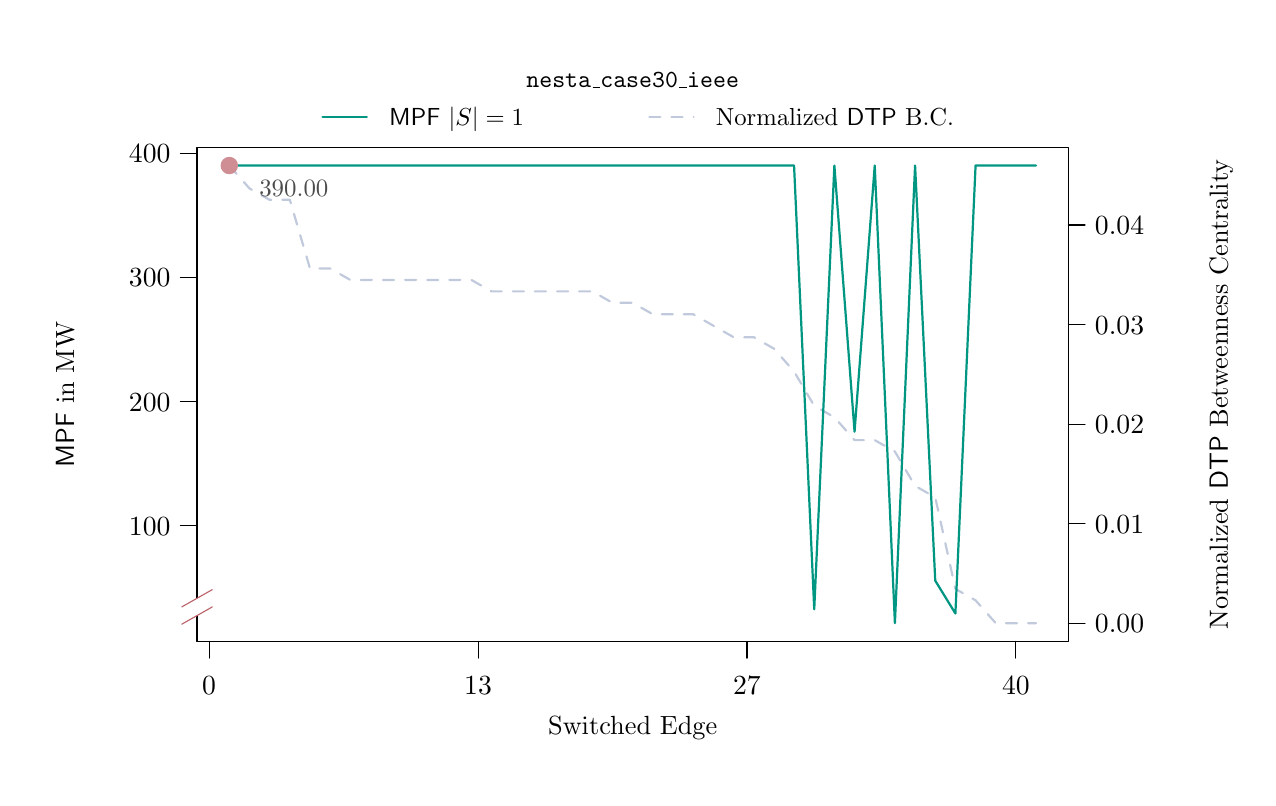
\begin{tikzpicture}[x=1pt,y=1pt]
\definecolor{fillColor}{RGB}{255,255,255}
\path[use as bounding box,fill=fillColor,fill opacity=0.00] (0,0) rectangle (440.85,271.01);
\begin{scope}
\path[clip] (  0.00,  0.00) rectangle (440.85,271.01);
\definecolor{drawColor}{RGB}{193,202,220}

\path[draw=drawColor,line width= 0.8pt,dash pattern=on 4pt off 4pt ,line join=round,line cap=round] ( 72.86,221.20) --
	( 80.15,212.93) --
	( 87.44,208.79) --
	( 94.73,208.79) --
	(102.01,183.99) --
	(109.30,183.99) --
	(116.59,179.85) --
	(123.88,179.85) --
	(131.17,179.85) --
	(138.45,179.85) --
	(145.74,179.85) --
	(153.03,179.85) --
	(160.32,179.85) --
	(167.61,175.72) --
	(174.89,175.72) --
	(182.18,175.72) --
	(189.47,175.72) --
	(196.76,175.72) --
	(204.05,175.72) --
	(211.34,171.58) --
	(218.62,171.58) --
	(225.91,167.45) --
	(233.20,167.45) --
	(240.49,167.45) --
	(247.78,163.31) --
	(255.06,159.18) --
	(262.35,159.18) --
	(269.64,155.04) --
	(276.93,146.78) --
	(284.22,134.37) --
	(291.50,130.24) --
	(298.79,121.97) --
	(306.08,121.97) --
	(313.37,117.83) --
	(320.66,105.43) --
	(327.95,101.30) --
	(335.23, 68.22) --
	(342.52, 64.08) --
	(349.81, 55.82) --
	(357.10, 55.82) --
	(364.39, 55.82);
\end{scope}
\begin{scope}
\path[clip] (  0.00,  0.00) rectangle (440.85,271.01);
\definecolor{drawColor}{RGB}{0,0,0}

\path[draw=drawColor,line width= 0.4pt,line join=round,line cap=round] ( 61.20, 49.20) --
	(376.05, 49.20) --
	(376.05,227.81) --
	( 61.20,227.81) --
	( 61.20, 49.20);
\end{scope}
\begin{scope}
\path[clip] (  0.00,  0.00) rectangle (440.85,271.01);
\definecolor{drawColor}{RGB}{0,0,0}

\path[draw=drawColor,line width= 0.4pt,line join=round,line cap=round] (376.05, 55.82) -- (376.05,199.70);

\path[draw=drawColor,line width= 0.4pt,line join=round,line cap=round] (376.05, 55.82) -- (382.05, 55.82);

\path[draw=drawColor,line width= 0.4pt,line join=round,line cap=round] (376.05, 91.79) -- (382.05, 91.79);

\path[draw=drawColor,line width= 0.4pt,line join=round,line cap=round] (376.05,127.76) -- (382.05,127.76);

\path[draw=drawColor,line width= 0.4pt,line join=round,line cap=round] (376.05,163.73) -- (382.05,163.73);

\path[draw=drawColor,line width= 0.4pt,line join=round,line cap=round] (376.05,199.70) -- (382.05,199.70);

\node[text=drawColor,anchor=base west,inner sep=0pt, outer sep=0pt, scale=  1.00] at (385.65, 52.37) {0.00};

\node[text=drawColor,anchor=base west,inner sep=0pt, outer sep=0pt, scale=  1.00] at (385.65, 88.34) {0.01};

\node[text=drawColor,anchor=base west,inner sep=0pt, outer sep=0pt, scale=  1.00] at (385.65,124.31) {0.02};

\node[text=drawColor,anchor=base west,inner sep=0pt, outer sep=0pt, scale=  1.00] at (385.65,160.28) {0.03};

\node[text=drawColor,anchor=base west,inner sep=0pt, outer sep=0pt, scale=  1.00] at (385.65,196.25) {0.04};
\end{scope}
\begin{scope}
\path[clip] (  0.00,  0.00) rectangle (440.85,271.01);
\definecolor{drawColor}{RGB}{0,150,130}

\path[draw=drawColor,line width= 0.8pt,line join=round,line cap=round] (106.55,238.60) -- (122.57,238.60);
\definecolor{drawColor}{RGB}{193,202,220}

\path[draw=drawColor,line width= 0.8pt,dash pattern=on 4pt off 4pt ,line join=round,line cap=round] (224.63,238.60) -- (240.65,238.60);
\definecolor{drawColor}{RGB}{0,0,0}

\node[text=drawColor,anchor=base,inner sep=0pt, outer sep=0pt, scale=  0.89] at (218.62,249.28) {\texttt{nesta\_case30\_ieee}};

\node[text=drawColor,anchor=base west,inner sep=0pt, outer sep=0pt, scale=  0.89] at (130.58,235.54) {$\mathsf{MPF}~|S|=1$};

\node[text=drawColor,anchor=base west,inner sep=0pt, outer sep=0pt, scale=  0.89] at (248.66,235.54) {Normalized~$\mathsf{DTP}$~B.C.};
\end{scope}
\begin{scope}
\path[clip] (  0.00,  0.00) rectangle (440.85,271.01);
\definecolor{drawColor}{RGB}{0,0,0}

\path[draw=drawColor,line width= 0.4pt,line join=round,line cap=round] ( 61.20, 90.98) -- ( 61.20,225.69);

\path[draw=drawColor,line width= 0.4pt,line join=round,line cap=round] ( 61.20, 90.98) -- ( 55.20, 90.98);

\path[draw=drawColor,line width= 0.4pt,line join=round,line cap=round] ( 61.20,135.88) -- ( 55.20,135.88);

\path[draw=drawColor,line width= 0.4pt,line join=round,line cap=round] ( 61.20,180.78) -- ( 55.20,180.78);

\path[draw=drawColor,line width= 0.4pt,line join=round,line cap=round] ( 61.20,225.69) -- ( 55.20,225.69);

\node[text=drawColor,anchor=base east,inner sep=0pt, outer sep=0pt, scale=  1.00] at ( 51.60, 87.53) {100};

\node[text=drawColor,anchor=base east,inner sep=0pt, outer sep=0pt, scale=  1.00] at ( 51.60,132.44) {200};

\node[text=drawColor,anchor=base east,inner sep=0pt, outer sep=0pt, scale=  1.00] at ( 51.60,177.34) {300};

\node[text=drawColor,anchor=base east,inner sep=0pt, outer sep=0pt, scale=  1.00] at ( 51.60,222.24) {400};
\end{scope}
\begin{scope}
\path[clip] (  0.00,  0.00) rectangle (440.85,271.01);
\definecolor{drawColor}{RGB}{255,255,255}
\definecolor{fillColor}{RGB}{255,255,255}

\path[draw=drawColor,line width= 0.4pt,line join=round,line cap=round,fill=fillColor] ( 55.69, 58.58) rectangle ( 66.71, 64.83);
\definecolor{drawColor}{RGB}{188,97,104}

\path[draw=drawColor,line width= 0.4pt,line join=round,line cap=round] ( 55.69, 55.45) -- ( 66.71, 61.70);

\path[draw=drawColor,line width= 0.4pt,line join=round,line cap=round] ( 55.69, 61.70) -- ( 66.71, 67.95);
\end{scope}
\begin{scope}
\path[clip] ( 61.20, 49.20) rectangle (376.05,227.81);
\definecolor{drawColor}{RGB}{0,150,130}

\path[draw=drawColor,line width= 0.8pt,line join=round,line cap=round] ( 72.86,221.20) --
	( 80.15,221.20) --
	( 87.44,221.20) --
	( 94.73,221.20) --
	(102.01,221.20) --
	(109.30,221.20) --
	(116.59,221.20) --
	(123.88,221.20) --
	(131.17,221.20) --
	(138.45,221.20) --
	(145.74,221.20) --
	(153.03,221.20) --
	(160.32,221.20) --
	(167.61,221.20) --
	(174.89,221.20) --
	(182.18,221.20) --
	(189.47,221.20) --
	(196.76,221.20) --
	(204.05,221.20) --
	(211.34,221.20) --
	(218.62,221.20) --
	(225.91,221.20) --
	(233.20,221.20) --
	(240.49,221.20) --
	(247.78,221.20) --
	(255.06,221.20) --
	(262.35,221.20) --
	(269.64,221.20) --
	(276.93,221.20) --
	(284.22, 60.87) --
	(291.50,221.20) --
	(298.79,125.02) --
	(306.08,221.20) --
	(313.37, 55.82) --
	(320.66,221.20) --
	(327.95, 71.19) --
	(335.23, 59.32) --
	(342.52,221.20) --
	(349.81,221.20) --
	(357.10,221.20) --
	(364.39,221.20);
\end{scope}
\begin{scope}
\path[clip] ( 61.20, 49.20) rectangle (376.05,227.81);
\definecolor{fillColor}{RGB}{207,142,147}

\path[fill=fillColor] ( 72.86,221.20) circle (  3.15);
\end{scope}
\begin{scope}
\path[clip] ( 61.20, 49.20) rectangle (376.05,227.81);
\definecolor{drawColor}{gray}{0.30}

\node[text=drawColor,anchor=base,inner sep=0pt, outer sep=0pt, scale=  0.90] at ( 96.18,210.04) {390.00};
\end{scope}
\begin{scope}
\path[clip] (  0.00,  0.00) rectangle (440.85,271.01);
\definecolor{drawColor}{RGB}{0,0,0}

\path[draw=drawColor,line width= 0.4pt,line join=round,line cap=round] ( 65.57, 49.20) -- (357.10, 49.20);

\path[draw=drawColor,line width= 0.4pt,line join=round,line cap=round] ( 65.57, 49.20) -- ( 65.57, 43.20);

\path[draw=drawColor,line width= 0.4pt,line join=round,line cap=round] (162.75, 49.20) -- (162.75, 43.20);

\path[draw=drawColor,line width= 0.4pt,line join=round,line cap=round] (259.92, 49.20) -- (259.92, 43.20);

\path[draw=drawColor,line width= 0.4pt,line join=round,line cap=round] (357.10, 49.20) -- (357.10, 43.20);

\node[text=drawColor,anchor=base,inner sep=0pt, outer sep=0pt, scale=  1.00] at ( 65.57, 30.00) {0};

\node[text=drawColor,anchor=base,inner sep=0pt, outer sep=0pt, scale=  1.00] at (162.75, 30.00) {13};

\node[text=drawColor,anchor=base,inner sep=0pt, outer sep=0pt, scale=  1.00] at (259.92, 30.00) {27};

\node[text=drawColor,anchor=base,inner sep=0pt, outer sep=0pt, scale=  1.00] at (357.10, 30.00) {40};

\node[text=drawColor,anchor=base,inner sep=0pt, outer sep=0pt, scale=  0.95] at (218.62, 15.60) {Switched Edge};

\node[text=drawColor,rotate= 90.00,anchor=base,inner sep=0pt, outer sep=0pt, scale=  0.95] at ( 16.80,138.51) {$\mathsf{MPF}$ in~$\mathrm{MW}$};

\node[text=drawColor,rotate= 90.00,anchor=base,inner sep=0pt, outer sep=0pt, scale=  0.95] at (433.65,138.51) {Normalized~$\mathsf{DTP}$ Betweenness Centrality};
\end{scope}
\end{tikzpicture}
